 
 
 
% 
% 
% 
% 
% 
%%%%%%%%%%%%%%%%%% 
%Disagreements, Philosophical and Otherwise
%%%%%%%%%%%%%%%%%% 
% 
% 
% 
% 
% 
\chapter{Disagreements, Philosophical and Otherwise}

\pubdata{Jennifer Lackey and David Christensen (eds.), \textit{Epistemology of Disagreement}, Oxford, 2013, 54-75. It has been improved by many comments from the editors.}

This paper started life as a short note I wrote around New Year 2007 while in Minneapolis. It was originally intended as a blog post. That might explain, if not altogether excuse, the flippant tone in places. But it got a little long for a post, so I made it into the format of a paper and posted it to my website. The paper has received a lot of attention, so it seems like it will be helpful to see it in print. Since a number of people have responded to the argument as stated, I've decided to just reprint the article warts and all, with a couple of clarifcatory footnotes added, and then after it I'll make a  few comments about how one of the key arguments was supposed to work, and how I see the overall argument of the note in the context of the subsequent debate.

\begin{Large}
\begin{center}
\textbf{Disagreeing about Disagreement (2007)}
\end{center}
\end{Large}

\noindent I argue with my friends a lot. That is, I offer them reasons to believe all sorts of philosophical conclusions. Sadly, despite the quality of my arguments, and despite their apparent intelligence, they don't always agree. They keep insisting on principles in the face of my wittier and wittier counterexamples, and they keep offering their own dull alleged counterexamples to my clever principles. What is a philosopher to do in these circumstances? (And I don't mean get better friends.)

One popular answer these days is that I should, to some extent, defer to my friends. If I look at a batch of reasons and conclude $p$, and my equally talented friend reaches an incompatible conclusion $q$, I should revise my opinion so I'm now undecided between $p$ and $q$. I should, in the preferred lingo, assign equal weight to my view as to theirs. This is despite the fact that I've looked at their reasons for concluding $q$ and found them wanting. If I hadn't, I would have already concluded $q$. The mere fact that a friend (from now on I'll leave off the qualifier 'equally talented and informed', since all my friends satisfy that) reaches a contrary opinion should be reason to move me. Such a position is defended by Richard Feldman \citeyearpar{Feldman2005-FELRTE, Feldman2006-FELEPA}, David Christensen \citeyearpar{Christensen2007-CHREOD} and Adam Elga \citeyearpar{Elga2007-ELGRAD}.

This equal weight view, hereafter EW, is itself a philosophical position. And while some of my friends believe it, some of my friends do not. (Nor, I should add for your benefit, do I.) This raises an odd little dilemma. If EW is correct, then the fact that my friends disagree about it means that I shouldn't be particularly confident that it is true, since EW says that I shouldn't be too confident about any position on which my friends disagree. But, as I'll argue below, to consistently implement EW, I have to be maximally confident that it is true. So to accept EW, I have to inconsistently both be very confident that it is true and not very confident that it is true. This seems like a problem, and a reason to not accept EW. We can state this argument formally as follows, using the notion of a peer and an expert. Some people are peers if they are equally philosophically talented and informed as each other, and one is more expert than another if they are more informed and talented than the other.

\begin{enumerate}
\item There are peers who disagree about EW, and there is no one who is an expert relative to them who endorses EW.
\item If 1 is true, then according to EW, my credence in EW should be less than 1.
\item If my credence in EW is less than 1, then the advice that EW offers in a wide range of cases is incoherent.
\item So, the advice EW offers in a wide range of cases is incoherent.
\end{enumerate}

The first three sections of this paper will be used to defend the first three premises. The final section will look at the philosophical consequences of the conclusion.

\section{Peers and EW}
Thomas Kelly \citeyearpar{Kelly2005-KELTES} has argued against EW and in favour of the view that a peer with the irrational view should defer to a peer with the rational view. Elga helpfully dubs this the 'right reasons' view. Ralph Wedgwood \citeyearpar[Ch. 11]{Wedgwood2007-WEDNON} has argued against EW and in favour of the view that one should have a modest 'egocentric bias', i.e. a bias towards one's own beliefs. On the other hand, as mentioned above, Elga, Christensen and Feldman endorse versions of EW. So it certainly looks like there are very talented and informed philosophers on either side of this debate.

Now I suppose that if we were taking EW completely seriously, we would at this stage of the investigation look very closely at whether these five really are epistemic peers. We could pull out their grad school transcripts, look at the citation rates for their papers, get reference letters from expert colleagues, maybe bring one or two of them in for job-style interviews, and so on. But this all seems somewhat inappropriate for a scholarly journal. Not to mention a little tactless.\footnote{Though if EW is correct, shouldn't the scholarly journals be full of just this information?}  So I'll just stipulate that they seem to be peers in the sense relevant for EW, and address one worry a reader may have about my argument.

An objector might say, ``Sure it seems antecedently that Kelly and Wedgwood are the peers of the folks who endorse EW. But take a look at the arguments for EW that have been offered. They look like good arguments, don't they? Doesn't the fact that Kelly and Wedgwood don't accept these arguments mean that, however talented they might be in general, they obviously have a blind spot when it comes to the epistemology of disagreement? If so, we shouldn't treat them as experts on this question.'' There is something right about this. People can be experts in one area, or even many areas, while their opinions are systematically wrong in another. But the objector's line is unavailable to defenders of EW.

Indeed, these defenders have been quick to distance themselves from the objector. Here, for instance, is Elga's formulation of the EW view, a formulation we'll return to below.

\begin{quote}Your probability in a given disputed claim should equal your prior conditional probability in that claim. Prior to what? Prior to your thinking through the claim, and finding out what your advisor thinks of it. Conditional on what? On whatever you have learned about the circumstances of how you and your advisor have evaluated the claim. \cite[490]{Elga2007-ELGRAD}
\end{quote}

The fact that Kelly and Wedgwood come to different conclusions can't be enough reason to declare that they are not peers. As Elga stresses, what matters is the prior judgment of their acuity. And Elga is right to stress this. If we declared anyone who doesn't accept reasoning that we find compelling not a peer, then the EW view will be trivial. After all, the EW view only gets its force from cases as described in the introduction, where our friends reject reasoning we accept, and accept reasons we reject. If that makes them not a peer, the EW view never applies. So we can't argue that anyone who rejects EW is thereby less of an expert in the relevant sense than someone who accepts it, merely in virtue of their rejection of EW. So it seems we should accept premise 1.

\section{Circumstances of Evaluation}
Elga worries about the following kind of case. Let $p$ be that the sum of a certain series of numbers, all of them integers, is 50. Let $q$ be that the sum of those numbers is $400e$. My friend and I both add the numbers, and I conclude $p$ while he concludes $q$. It seems that there is no reason to defer to my friend. I know, after all, that he has made some kind of mistake. The response, say defenders of EW, is that deference is context-sensitive. If I know, for example, that my friend is drunk, then I shouldn't defer to him. More generally, as Elga puts it, how much I should defer should depend on what I know about the circumstances.

Now this is relevant because one of the relevant circumstances might be that my friend has come to a view that I regard as insane. That's what happens in the case of the sums. Since my prior probability that my friend is right given that he has an insane seeming view is very low, my posterior probability that my friend is right should also, according to Elga, be low. Could we say that, although antecedently we regard Wedgwood and Kelly as peers of those they disagree with, that the circumstance of their disagreement is such that we should disregard their views?

It is hard to see how this would be defensible. It is true that a proponent of EW will regard Kelly and Wedgwood as wrong. But we can't say that we should disregard the views of all those we regard as mistaken. That leads to trivialising EW, for reasons given above. The claim has to be that their views are so outrageous, that we wouldn't defer to anyone with views that outrageous. And this seems highly implausible. But that's the only reason that premise 2 could be false. So we should accept premise 2.

\section{A Story about Disagreement}
The tricky part of the argument is proving premise 3. To do this, I'll use a story involving four friends, Apollo, Telemachus, Adam and Tom. The day before our story takes place, Adam has convinced Apollo that he should believe EW, and organise his life around it. Now Apollo and Telemachus are on their way to Fenway Park to watch the Red Sox play the Indians. There have been rumours flying around all day about whether the Red Sox injured star player, David Ortiz, will be healthy enough to play. Apollo and Telemachus have heard all the competing reports, and are comparing their credences that Ortiz will play. (Call the proposition that he will play $p$.) Apollo's credence in $p$ is 0.7, and Telemachus's is 0.3. In fact, 0.7 is the rational credence in $p$ given their shared evidence, and Apollo truly believes that it is.\footnote{This is obviously somewhat of an idealisation, since there won't usually be a unique precise rational response to the evidence. But I don't think this idealisation hurts the argument to follow. I should note that the evidence here \textit{excludes} their statements of their credences, so I really mean the evidence that they brought to bear on the debate over whether $p$.}  And, as it turns out, the Red Sox have decided but not announced that Ortiz will play, so $p$ is true.

Despite these facts, Apollo lowers his credence in $p$. In accord with his newfound belief in EW, he changes his credence in $p$ to 0.5. Apollo is sure, after all, that when it comes to baseball Telemachus is an epistemic peer. At this point Tom arrives, and with a slight disregard for the important baseball game at hand, starts trying to convince them of the right reasons view on disagreement. Apollo is not convinced, but Telemachus thinks it sounds right. As he puts it, the view merely says that the rational person believes what the rational person believes. And who could disagree with that?

Apollo is not convinced, and starts telling them the virtues of EW. But a little way in, Tom cuts him off with a question. ``How probable,'' he asks Apollo, ``does something have to be before you'll assert it?'' 

Apollo says that it has to be fairly probable, though just what the threshold is depends on just what issues are at stake.  But he agrees that it has to be fairly high, well above 0.5 at least.

``Well,'' says Tom, ``in that case you shouldn't be defending EW in public. Because you think that Telemachus and I are the epistemic peers of you and Adam. And we think EW is false. So even by EW's own lights, the probability you assign to EW should be 0.5. And that's not a high enough probability to assert it.'' Tom's speech requires that Apollo regard he and Telemachus as Apollo's epistemic peers with regard to this question. By premises 1 and 2, Apollo should do this, and we'll assume that he does.

So Apollo agrees with all this, and agrees that he shouldn't assert EW any more. But he still plans to use it, i.e. to have a credence in $p$ of 0.5 rather than 0.7. But now Telemachus and Tom press on him the following analogy.

Imagine that there were two competing experts, each of whom gave differing views about the probability of $q$. One of the experts, call her Emma, said that the probability of $q$, given the evidence, is 0.5. The other expert, call her Rae, said that the probability of $q$, given the evidence, is 0.7. Assuming that Apollo has the same evidence as the experts, but he regards the experts as experts at evaluating evidence, what should his credence in $q$ be? It seems plausible that it should be a weighted average of what Emma says and what Rae says. In particular, it should be 0.5 only if Apollo is maximally confident that Emma is the expert to trust, and not at all confident that Rae is the expert to trust.

The situation is parallel to the one Apollo actually faces. EW says that his credence in $p$ should be 0.5. The right reason view says that his credence in $p$ should be 0.7. Apollo is aware of both of these facts.\footnote{Added in 2011: This is a bit quick. I think I was assuming here that Apollo adopts of a version of EW where conflicting peer judgments don't \textit{defeat} the support his evidence provides for $p$, but rather \textit{screen} it off. So he could take EW as given, and still know that given merely the evidence he had before talking to Telemachus, the rational credence in $p$ is 0.7. That's not, on Apollo's view, the rational credence in $p$ given \textit{all} his evidence, because Telemachus's judgment counts for a lot. But it is the rational credence given initial evidence, and he knows that even after talking to Telemachus. Since the rational credence given his initial evidence just is the credence the right reasons view recommends, he knows it is what the right reasons view recommends. Or, at least, he knows it is what the right reasons view recommends on the view that opposing judgments screen off underlying evidence. But Apollo could hold the EW view without holding that view about screening. If Apollo thinks that Telemachus's judgment \textit{defeats} his initial reasons for thinking the rational credence in $p$ given his (prior) evidence is 0.7, then he won't know what right reasons recommends. Thanks here to David Christensen.} So his credence in $p$ should be 0.5 iff he is certain that EW is the theory to trust, just as his credence in $q$ should be 0.5 iff he is certain that Emma is the expert to trust. Indeed, a credence of 0.5 in $p$ is incoherent unless Apollo is certain EW is the theory to trust. But Apollo is not at all certain of this. His credence in EW, as is required by EW itself, is 0.5. So as long as Apollo keeps his credence in p at 0.5, he is being incoherent. But EW says to keep his credence in p at 0.5. So EW advises him to be incoherent. That is, EW offers incoherent advice. We can state this more carefully in an argument.

\begin{enumerate}
\setcounter{enumi}{4}
\item EW says that Apollo's credence in p should be 0.5.
\item If 5, then EW offers incoherent advice unless it also says that Apollo's credence in EW should be 1.
\item EW says that Apollo's credence in EW should be 0.5.
\item So, EW offers incoherent advice.
\end{enumerate}

\noindent Since Apollo's case is easily generalisable, we can infer that in a large number of cases, EW offers advice that is incoherent. Line 7 in this argument is hard to assail given premises 1 and 2 of the master argument. But I can imagine objections to each of the other lines.

\medskip \noindent \textit{Objection}: Line 6 is false. Apollo can coherently have one credence in p while being unsure about whether it is the rational credence to have. In particular, he can coherently have his credence in p be 0.5, while he is unsure whether his credence in p should be 0.5 or 0.7. In general there is no requirement for agents who are not omniscient to have their credences match their judgments of what their credences should be.

\smallskip \noindent \textit{Replies}: I have two replies to this, the first dialectical and the second substantive.

The dialectical reply is that if the objector's position on coherence is accepted, then a lot of the motivation for EW fades away. A core idea behind EW is that Apollo was unsure before the conversation started whether he or Telemachus would have the most rational reaction to the evidence, and hearing what each of them say does not provide him with more evidence. (See the 'bootstrapping' argument in \citet{Elga2007-ELGRAD} for a more formal statement of this idea.) So Apollo should have equal credence in the rationality of his judgment and of Telemachus's judgment.

But if the objector is correct, Apollo can do that without changing his view on EW one bit. He can, indeed should, have his credence in $p$ be 0.7, while being uncertain whether his credence in p should be 0.7 (as he thinks) or 0.3 (as Telemachus thinks). Without some principle connecting what Apollo should think about what he should think to what Apollo should think, it is hard to see why this is not the uniquely rational reaction to Apollo's circumstances. In other words, if this is an objection to my argument against EW, it is just as good an objection to a core argument for EW.

The substantive argument is that the objector's position requires violating some very weak principles concerning rationality and higher-order beliefs. The objector is right that, for instance, in order to justifiably believe that $p$ (to degree $d$), one need not know, or even believe, that one is justified in believing $p$ (to that degree). If nothing else, the anti-luminosity arguments in \citet{Williamson2000-WILKAI} show that to be the case. But there are weaker principles that are more plausible, and which the objector's position has us violate. In particular, there is the view that we can't both be justified in believing that $p$ (to degree $d$), while we know we are not justified in believing that we are justified in believing $p$ (to that degree). In symbols, if we let $Jp$ mean that the agent is justified in believing $p$, and box and diamond to be epistemic modals, we have the principle \textbf{MJ} (for Might be Justified).

\begin{description}
\item[MJ] $Jp \rightarrow \diamond JJp$
\end{description}

This seems like a much more plausible principle, since if we know we aren't justified in believing we're justified in believing $p$, it seems like we should at least suspend judgment in $p$. That is, we shouldn't believe $p$. That is, we aren't justified in believing $p$. But the objector's position violates principle \textbf{MJ}, or at least a probabilistic version of it, as we'll now show.

We aim to prove that the objector is committed to Apollo being justified in believing $p$ to degree 0.5, while he knows he is not justified in believing he is justified in believing $p$ to degree 0.5. The first part is trivial, it's just a restatement of the objector's view, so it is the second part that we must be concerned with. 

Now, either EW is true, or it isn't true. If it is true, then Apollo is not justified in having a greater credence in it than 0.5. But his only justification for believing p to degree 0.5 is EW. He's only justified in believing he's justified in believing $p$ if he can justify his use of EW in it. But you can't justify a premise in which your rational credence is 0.5. So Apollo isn't justified in believing he is justified in believing $p$. If EW isn't true, then Apollo isn't even justified in believing $p$ to degree 0.5. And he knows this, since he knows EW is his only justification for lowering his credence in $p$ that far. So he certainly isn't justified in believing he is justified in believing $p$ to degree 0.5 Moreover, every premise in this argument has been a premise that Apollo knows to obtain, and he is capable of following all the reasoning. So he knows that he isn't justified in believing he is justified in believing $p$ to degree 0.5, as required.

The two replies I've offered to the objector complement one another. If someone accepts \textbf{MJ}, then they'll regard the objector's position as incoherent, since we've just shown that \textbf{MJ} is inconsistent with that position. If, on the other hand, someone rejects \textbf{MJ} and everything like it, then they have little reason to accept EW in the first place. They should just accept that Apollo's credence in p should be, as per hypothesis the evidence suggests, 0.7. The fact that an epistemic peer disagrees, in the face of the same evidence, might give Apollo reason to doubt that this is in fact the uniquely rational response to the evidence. But, unless we accept a principle like \textbf{MJ}, that's consistent with Apollo retaining the rational response to the evidence, namely a credence of 0.7 in p. So it is hard to see how someone could accept the objector's argument, while also being motivated to accept EW. In any case, I think \textbf{MJ} is plausible enough on its own to undermine the objector's position.\footnote{Added in 2011: I still think there's a dilemma here for EW, but I'm less convinced than I used to be that \textbf{MJ} is correct. In particular, \textbf{MJ} seems a little too close to the `ratificationist' views I attack in section 6 to be confident that it is true.}

\medskip \noindent \textit{Objection}: Line 5 is false. Once we've seen that the credence of EW is 0.5, then Apollo's credence in first-order claims such as p should, as the analogy with q suggests, be a weighted average of what EW says it should be, and what the right reason view says it should be. So, even by EW's own lights, Apollo's credence in p should be 0.6.

\smallskip \noindent \textit{Replies}: Again I have a dialectical reply, and a substantive reply.

The dialectical reply is that once we make this move, we really have very little motivation to accept EW. There is, I'll grant, some intuitive plausibility to the view that when faced with a disagreeing peer, we should think the right response is half way between our competing views. But there is no intuitive plausibility whatsoever to the view that in such a situation, we should naturally move to a position three-quarters of the way between the two competing views, as this objector suggests. Much of the argument for EW, especially in Christensen, turns on intuitions about cases, and the objector would have us give all of that up. Without those intuitions, however, EW falls in a heap.

The substantive reply is that the idea behind the objection can't be coherently sustained. The idea is that we should first apply EW to philosophical questions to work out the probability of different theories of disagreement, and then apply those probabilities to first-order disagreements. The hope is that in doing so we'll reach a stable point at which EW can be coherently applied. But there is no such stable point. Consider the following series of questions.

\begin{description}
\item[Q1] Is EW true?
\end{description}

\noindent Two participants say yes, two say no. We have a dispute, leading to our next question.

\begin{description}
\item[Q2] What is the right reaction to the disagreement over Q1?
\end{description}

\noindent EW answers this by saying our credence in EW should be 0.5. But that's not what the right reason proponents say. They don't believe EW, so they have no reason to move their credence in EW away from 0. So we have another dispute, and we can ask

\begin{description}
\item[Q3] What is the right reaction to the disagreement over Q2?
\end{description}

\noindent EW presumably says that we should again split the difference. Our credence in EW might now be 0.25, half-way between the 0.5 it was after considering Q2, and what the right reasons folks say. But, again, those who don't buy EW will disagree, and won't be moved to adjust their credence in EW. So again there's a dispute, and again we can ask

\begin{description}
\item[Q4] What is the right reaction to the disagreement over Q3?
\end{description}

\noindent This could go on for a while. The only 'stable point' in the sequence is when we assign a credence of 0 to EW. That's to say, the only way to coherently defend the idea behind the objection is to assign credence 0 to EW. But that's to give up on EW. As with the previous objection, we can't hold on to EW and object to the argument.

\section{Summing Up}
The story I've told here is a little idealised, but otherwise common enough. We often have disagreements both about first-order questions, and about how to resolve this disagreement. In these cases, there is no coherent way to assign equal weight to all prima facie rational views both about the first order question and the second order, epistemological, question. The only way to coherently apply EW to all first order questions is to put our foot down, and say that despite the apparent intelligence of our philosophical interlocutors, we're not letting them dim our credence in EW. But if we are prepared to put our foot down here, why not about some first-order question or other? It certainly isn't because we have more reason to believe an epistemological theory like EW than we have to believe first order theories about which there is substantive disagreement. So perhaps we should hold on to those theories, and let go of EW. 

\begin{Large}
\begin{center}
\textbf{Afterthoughts (2011)}
\end{center}
\end{Large}

\section{The Regress Argument}

The argument at the end of section 3 is too condensed. There are a couple of distinct arguments that need disentangling. One concerns stubborn interlocutors, the other concerns whether the EW theory is believable.

Here's a simple version of the stubborn interlocutors argument. After they hear each other's views, Apollo's credence in $p$ goes to 0.5, but Tele\-machus's credence stays at 0.3. Well, Apollo and Telemachus are peers, so by EW now Apollo's credence should be half-way between these two values. That is, it should be 0.4. But at the time Apollo forms this credence, he and Telemachus are peers, who have the same evidence and have acted on it to the fullest extent of their ability. So Apollo, if he believes in EW, should move his credence to 0.35, and so on until he fully concedes to Telemachus. But it is absurd that EW should force complete concession to a stubborn interlocutor, so EW is false.

Now there are a couple of things one might say to that argument. Perhaps one will reject the last step, and deny that it is a \textit{reductio} of EW. Perhaps one will say that there's a principled reason to apply EW \textit{once}. I don't think either will work, but they do seem like the most attractive ways out of this problem. We'll return to this below, after looking at the other thread of the regress argument.

Arguably, Apollo should have credences that are justifiable by his own lights. And that requires that his credences be in some kind of equilibrium. But many credences won't satisfy this requirement. Let's say that his credence in both $p$ and in EW is 0.5. Then he doesn't have any justification for having a credence 0.5 in $p$. After all, he has already conceded that he can only justify having a credence of 0.5 in $p$ if he is certain that EW is true. But he can't be certain that EW is true, since it is subject to peer disagreement.

So what kind of state would be an equilibrium for Apollo? This question requires a little care. Say a $0^{th}$ order proposition is a proposition that is in no way about what to do when faced with a disagreement. Say that a $(k+1)^{th}$ order proposition is one that is about how to resolve disagreements about $k^{th}$ order propositions. We'll assume for simplicity that the only options on the table are the right reasons view and EW. I doubt doing this will significantly stack the deck in my favour, though I don't have much of a proof of this. 

We can carve up the equal weight view and the right reasons view into a number of different sub-views. The $n^{th}$ order equal weight view (for $n \geq 1$) says that when faced with a disagreement about $(n-1)^{th}$ order propositions, one should assign equal weight to the credences of each peer. The $n^{th}$ order right reasons view, by contrast, says that one should assign no weight to the credences of the peers, and just follow the reasons where they lead, when faced with such a disagreement. This way of stating things makes it clear that one consistent view is to hold the first order equal weight view, and the right reasons view for second and higher orders. Indeed, such a view is defended by Adam Elga \citeyearpar{Elga2010-ELGHTD}.

Now we need an equilibrium condition on credal states. Let $r$ be an $n^{th}$ order proposition, for any $n \geq 0$. Assume that the agent believes that the $(n+1)^{th}$ order equal weight view recommends assigning credence $x_E$ to $r$, and the $(n+1)^{th}$ order right reasons view recommends assigning credence $x_R$ to $r$. Finally, assume that the agent's credence in the $(n+1)^{th}$ order equal weight view is $y$, and hence their credence in the $(n+1)^{th}$ order right reasons view is $1-y$. Then the equilibrium condition is that their credence in $r$ is $x_Ey + x_R(1-y)$. If that's not their credence in $r$, then they aren't treating their philosophical views as experts, so there is a disequilibrium between their lower-order and higher-order beliefs.

Now let $f$ be a function from non-negative integers into [0, 1] such that $f(0)$ is Apollo's credence in $p$, and $f(n)$ is his credence in the $n^{th}$ order equal weight view. Apollo thinks the reasons in favour of the equal weight view are good, so for any $n \geq 1$, he thinks the $(n+1)^{th}$ order right reasons view recommends having some higher credence, call it $x$, in the $n^{th}$ order equal weight view.\footnote{I think $x$ should be 1. That's because Apollo starts off with credence 1 in the $n^{th}$ order equal weight view, and conditional on the right reasons view being correct, he doesn't have any reason to deviate from that because someone disagrees. But this doesn't seem to persuade a lot of people. And while I don't think failure to persuade is evidence of falsity, it is evidence of failure of persuasiveness. And I like my arguments to be persuasive. So I won't assume $x = 1$.}
 But he knows his peers disagree, so he thinks the $(n+1)^{th}$ order equal weight  view recommends having credence 0.5 in the $n^{th}$ order equal weight view. And of course things are a little different at the base level, where the first order equal weight view recommends credence 0.5 in $p$, and the first order right reasons view recommends some other credence $y$ in $p$.\footnote{For reasons given in the previous footnote, I think $y = 0.7$, but I won't assume that here. I will assume $y \leq 0.7$, since it is hard to see how that could be violated.} So we need an $f$ with the following features:
\begin{align}
f(0) &= 0.5f(1) + y(1-f(1)) \\
&\text{while for } n \geq 1\\
f(n) &= 0.5f(n+1) + x(1-f(n+1)) \\
&= x + (0.5-x)f(n+1)
\end{align}
\noindent Now let's find the values of $f, x, y$ such that the minimal value of $f(n)$ is maximised (for $n> 0$). I'm assuming here that the full equal weight view is the conjunction of each of the orders of equal weight views, and the credence in a conjunction is no greater than the minimal value of a credence in the conjuncts. Note that if $f(k+1) > \nicefrac{2}{3}$, then $f(k) < \nicefrac{2}{3}$, since 
\begin{align}
f(k) &= 0.5f(k+1) + x(1-f(k+1)) \\
&\leq 0.5f(k+1) + 1-f(k+1) \\
&= 1 - 0.5f(k+1) \\
&< \nicefrac{2}{3}
\end{align}
\noindent So the best case scenario, if our aim is to maximise the minimal value of $f(n)$ is that $x=1$, and $f(n) = \nicefrac{2}{3}$ for all $n>0$, while $f(0) = \nicefrac{1+y}{3}$. That is, the highest credence that can coherently be held in EW is $\nicefrac{2}{3}$.

Now that isn't a great conclusion, since a theory that says if you accept the arguments for it are completely compelling, you should still only give it credence $\nicefrac{2}{3}$ is not looking too great. But it is different from the earlier conclusion. The stubborn interlocutors argument said that an EW theorist should completely concede to a stubborn interlocutor. A special case of this is that if we are faced with a stubborn interlocutor, our credence in EW goes to 0. The `equiibrium' argument I've just been running, on the other hand, says that when faced with \textit{any} disagreeing peer, even not a stubborn one, one's credence in EW should fall far enough that one no longer believes EW. I think the argument at the end of section 3 of the original paper runs together the equilibrium argument and the stubborn interlocutors argument.

One could resist the equilibrium argument by denying that it is a requirement of rationality that one's credences be in this kind of equilibrium. For what it's worth, I don't think that it is a requirement of rationality that one's credences be in this kind of equilibrium. But it is hard to square that denial with many of the motivations for EW. So I think most EW defenders won't want to do that. We'll come back to this point, in effect, in the next section.

Interestingly, one other natural response to the argument is to say that the right credence in the second order right reasons view is 1. That is, in effect, the line that Adam Elga takes in his \citeyearpar{Elga2010-ELGHTD}. In the terms we have here, we end up with $f(0) = 0.5, f(1) = 1, f(n) = 0$ for $n \geq 2$. That gives up on the full version of EW, but maybe it is enough to rescue the first order version. And, interestingly, it might provide a way out of the stubborn interlocutor argument. If $f(2) = 1$, then perhaps we can take Telemachus's unwillingness to adjust his credences in the light of disagreement to be a sign that he isn't Apollo's peer when it comes to debates about second order propositions. So Apollo need not keep adjusting his credences, because he need not keep regarding Telemachus as a peer. Now we could question whether treating first order and higher order equal weight so differently is well justified.  And we could question whether this approach to the stubborn interlocutor question is really consistent with the general attitude towards peerhood that EW proponents adopt. But I don't want to get into those debates \textit{here}. Rather, I just wanted to separate out two different strands in the regress argument from the end of section 3, two strands that are excessively blurred in the original note.

\section{The Philosophical Significance of Philosophical Disagreements}

\noindent I now think that the kind of argument I presented in the 2007 paper is not really an argument against EW as such, but an argument against one possible motivation for EW. I also think that alternate motivations for EW are no good, so I still think it is an important argument. But I think its role in the dialectic is a little more complicated than I appreciated back then.

Much of my thinking about disagreement problems revolves around the following table. The idea behind the table, and much of the related argument, is due to Thomas Kelly \citeyearpar{Kelly2010-KELPDA}. In the table, $S$ and $T$ antecedently had good reasons to take themselves to be epistemic peers, and they know that their judgments about $p$ are both based on $E$. In fact, $E$ is excellent evidence for $p$, but only $S$ judges that $p$; $T$ judges that $\neg p$. Now let's look at what seems to be the available evidence for and against $p$.

\begin{center}
\begin{tabular}{c c}
\textbf{Evidence for $p$} & \textbf{Evidence against $p$} \\
$S$'s judgment that $p$ & $T$'s judgment that $\neg p$ \\
$E$ & \\
\end{tabular}
\end{center}

\noindent Now that doesn't look to me like a table where the evidence is equally balanced for and against $p$. Even granting that the judgments are evidence over and above $E$, and granting that how much weight we should give to judgments should track our \textit{ex ante} judgments of their reliability rather than our \textit{ex post} judgments of their reliability, both of which strike me as false but necessary premises for EW, it \textit{still} looks like there is more evidence for $p$ than against $p$.\footnote{By \textit{ex ante} and \textit{ex post} I mean before and after we learn about $S$ and $T$'s use of $E$ to make a judgment about $p$. I think that should change how reliable we take $S$ and $T$ to be, and that this should matter to what use, if any, we put their judgments, but it is crucial to EW that we ignore this evidence. Or, at least, it is crucial to EW that $S$ and $T$ ignore this evidence.} There is strictly more evidence for $p$ than against it, since $E$ exists. If we want to conclude that $S$ should regard $p$ and $\neg p$ as equally well supported for someone in her circumstance, we have to show that the table is somehow wrong. I know of three possible moves the EW defender could make here.

David Christensen \citeyearpar{Christensen2010-CHRDQB}, as I read him, says that the table is wrong because when we are representing the evidence $S$ has, we should not include her own judgment. There's something plausible to this. Pretend for a second that $T$ doesn't exist, so it's clearly rational for $S$ to judge that $p$. It would still be wrong of $S$ to say, ``Since $E$ is true, $p$. And I judged that $p$, so that's another reason to believe that $p$, because I'm smart.'' By hypothesis, $S$ is smart, and that smart people judge things is reason to believe those things are true. But this doesn't work when the judgment is one's own. This is something that needs explaining in a full theory of the epistemic significance of judgment, but let's just take it as a given for now.\footnote{My explanation is that evidence screens any judgments made on the basis of that evidence, in the sense of screening to be described below.} Now the table, or at least the table as is relevant to $S$, looks as follows.

\begin{center}
\begin{tabular}{c c}
\textbf{Evidence for $p$} & \textbf{Evidence against $p$} \\
$E$ & $T$'s judgment that $\neg p$ \\
\end{tabular}
\end{center}

\noindent But I don't think this does enough to support EW, or really anything like it. First, it won't be true in general that the two sides of this table balance. In many cases, $E$ is strong evidence for $p$, and $T$'s judgment won't be particularly strong evidence against $p$. In fact, I'd say the kind of case where $E$ is much better evidence for $p$ than $T$'s judgment is against $p$ is the statistically normal kind. Or, at least, it is the normal kind of case modulo the assumption that $S$ and $T$ have the same evidence. In cases where that isn't true, learning that $T$ thinks $\neg p$ is good evidence that $T$ has evidence against $p$ that you don't have, and you should adjust accordingly. But by hypothesis, $S$ knows that isn't the case here. So I don't see why this should push us even close to taking $p$ and $\neg p$ to be equally well supported.

The other difficulty for defending EW by this approach is that it seems to undermine the original motivations for the view. As Christensen notes, the table above is specifically for $S$. Here's what the table looks like for $T$.

\begin{center}
\begin{tabular}{c c}
\textbf{Evidence for $p$} & \textbf{Evidence against $p$} \\
$S$'s judgment that $p$ & \\
$E$ & \\
\end{tabular}
\end{center}

\noindent It's no contest! So $T$ should firmly believe $p$. But that's not a way of saying the two peers should have \textit{equal} weight. Instead, it looks like a way of saying that, at least in this case, the right reasons view is right; $T$ should simply follow the evidence, and believe as if the disagreement never happened. Obviously there are going to be many views that say that the right reasons view happens to correlate with the right answer in this case without being generally correct. (The right reasons view, to this way of thinking, has the virtues of a clock stopped at the correct time.) So this isn't an argument for right reasons. But it does seem to undermine strong versions of equal weight.

The second approach to blocking the table is to say that $T$'s judgment is an undercutting defeater for the support $E$ provides for $p$. This looks superficially promising. Having a smart person say that your evidence supports something other than you thought it did seems like it could be an undercutting defeater, since it is a reason to think the evidence supports something else, and hence doesn't support what you thought it does. And, of course, if $E$ is undercut, then the table just has one line on it, and the two sides look equal.

But it doesn't seem like it can work in general, for a reason that \citet{Kelly2010-KELPDA} makes clear. We haven't said what $E$ is so far. Let's start with a case where $E$ consists of the judgments of a million other very smart people that $p$. Then no one, not even the EW theorist, will think that $T$'s judgment undercuts the support $E$ provides to $p$. Indeed, even if $E$ just consists of one other person's judgment, it won't be undercut by $T$'s judgment. The natural thought for an EW-friendly person to have in that case is that since there are two people who think $p$, and one who thinks $\neg p$, then $S$'s credence in $p$ should be $\nicefrac{2}{3}$. But that's impossible if $E$, i.e., the third person's judgment, is undercut by $T$'s judgment. It's true that $T$'s judgment will partially \textit{rebut} the judgments that $S$, and the third party, make. It will move the probability of $p$, at least according to EW, from 1 to $\nicefrac{2}{3}$. But that evidence won't be in any way \textit{undercut}.

And as Kelly points out, evidence is pretty fungible. Whatever support $p$ gets from other people's judgments, it could get very similar support from something other than a judgment. We get roughly the same evidence for $p$ by learning that a smart person predicts $p$ as learning that a successful computer model predicts $p$. So the following argument looks sound to me.

\begin{enumerate}
\item When $E$ consists of other people's judgments, the support it provides to $p$ is not undercut by $T$'s judgment.
\item If the evidence provided by other people's judgments is not undercut by $T$'s judgment, then some non-judgmental evidence is not undercut by $T$'s judgment.
\item So, not all non-judgmental evidence is not undercut by $T$'s judgment.
\end{enumerate}

\noindent So it isn't true in general that the table is wrong because $E$ has been defeated by an undercutting defeater.

There's another problem with the defeat model in cases where the initial judgments are not full beliefs. Change the case so $E$ provides basically no support to either $p$ or $\neg p$. Here's one case where that might happen.\footnote{This is a variant of a case Ishani Maitra uses for a different purpose.} $S$ and $T$ are two old blowhards discussing an upcoming football match, as it turns out a cup final, between two teams about which they know next to nothing. All that they know is that one of the teams is full of players with `big match experience', and the other team isn't. Both $S$ and $T$ are aware that there are mountains of studies showing no correlation between big match experience and success in cups. But they dismiss these because, well, what would pointy-headed stats geeks know about winning a cup? Let $E$ be what they know about the two teams, and $p$ be the proposition that the team with the big match experience will win. $S$ doesn't think there's enough reason to believe $p$, since they know so little about the teams, while $T$ thinks the big match experience will be enough, so $p$ will be true. Also assume that $S$ and $T$ are peers; they know that they have a similar, and similarly bad, track record at predicting these kinds of games. Here's the table then:

\begin{center}
\begin{tabular}{c c}
\textbf{Evidence for $p$} & \textbf{Evidence against $p$} \\
$T$'s judgment that $p$ & \\
\end{tabular}
\end{center}

\noindent Since $E$ is irrelevant, it doesn't appear, either before or after we think about defeaters. And since $T$ is not very competent, that's not great evidence for $p$. But EW says that $S$ should `split the difference' between her initial agnositicism, and $T$'s firm belief in $p$. I don't see how that could be justified by $S$'s evidence.

So that move doesn't work either, and we're left with the third option for upsetting the table. This move is, I think, the most promising of the lot. It is to say that $S$'s own judgment \textit{screens off} the evidence that $E$ provides. So the table is misleading, because it `double counts' evidence.

The idea of screening I'm using here, at least on behalf of EW, comes from Reichenbach's \textit{The Direction of Time}, \nocite{Reichenbach1956} and in particular from his work on deriving a principle that lets us infer events have a common cause. The notion was originally introduced in probabilistic terms. We say that \(C\) screens off the positive correlation between \(B\) and \(A\) if the following two conditions are met.

\begin{enumerate}
\item \(A\) and \(B\) are positively correlated probabilistically, i.e. \(Pr(A | B) > Pr(A)\).
\item  Given \(C\), \(A\) and \(B\) are probabilistically independent, \\ i.e. \(Pr(A | B \wedge C) = Pr(A | C)\).
\end{enumerate}

\noindent I'm interested in an evidential version of screening. If we have a probabilistic analysis of evidential support, the version of screening I'm going to offer here is identical to the Reichenbachian version just provided. But I want to stay neutral on whether we should think of evidence probabilistically.\footnote{In general I'm sceptical of always treating evidence probabilistically. Some of my reasons for scepticism are in \citet{Weatherson2007}.} When I say that \(C\) screens off the evidential support that \(B\) provides to \(A\), I mean the following. (Both these clauses, as well as the statement that \(C\) screens off \(B\) from \(A\), are made relative to an evidential background. I'll leave that as tacit in what follows.)

\begin{enumerate}
\item \(B\) is evidence that \(A\).
\item  \(B \wedge C\) is no better evidence that \(A\) than \(C\) is.\footnote{Branden Fitelson pointed out to me that the probabilistic version entails one extra condition, namely that  \(\neg B \wedge C\) is no worse evidence for \(A\) than \(C\) is. But I think that extra condition is irrelevant to disagreement debates, so I'm leaving it out.}
\end{enumerate}

\noindent Here is one stylised example of where screening helps conceptualise things. Detective Det is trying to figure out whether suspect Sus committed a certain crime. Let \(A\) be that Sus is guilty, \(B\) be that Sus was seen near the crime scene near the time the crime was committed, and \(C\) be that Sus was at the crime scene when the crime was committed. Then both clauses are satisfied. \(B\) is evidence for \(A\); that's why we look for witnesses who place the suspect near the crime scene. But given the further evidence \(C\), then \(B\) is neither here nor there with respect to \(A\). We're only interested in finding if Sus was near the crime scene because we want to know whether he was at the crime scene. If we know that he was there, then learning he was seen near there doesn't move the investigation along. So both clauses of the definition of screening are satisfied.

When there is screened evidence, there is the potential for double counting. It would be wrong to say that if we know $B \wedge C$ we have two pieces of evidence against Sus. Similarly, if a judgment screens off the evidence it is based on, then the table `double counts' the evidence for $p$. Removing the double counting, by removing $E$, makes the table symmetrical. And that's just what EW needs.

So the hypothesis that judgments screen the evidence they are based on, or JSE for short, can help EW respond to the argument from this table. And I think it gets the right results in the puzzle cases mentioned above. It helps with the `cup final' case, because it says that since $T$ has such a poor track record, $S$ shouldn't be confident in $p$ on the basis of $T$'s judgment. It provides a principled reason why the number of peers on either side of a disagreement matters, since it denies that conflicting judgments are defeaters for each of the peers. And it explains why even the mistaken party should `split the difference' rather than concede to the other person, since the evidence $E$ that would motivate a concession has been screened off. So I think it's an attractive way forward for EW.

But JSE is vulnerable to regress arguments. I now think that the argument in `Disagreeing about Disagreement' is a version of the regress argument against JSE. So really it's an argument against the most promising response to a particularly threatening argument against EW.

Unfortunately for EW, those regress arguments are actually quite good. To see ths, let's say an agent makes a judgment on the basis of \(E\), and let \(J\) be the proposition that that judgment was made. JSE says that \(E\) is now screened off, and the agent's evidence is just \(J\). But with that evidence, the agent presumably makes a new judgment. Let \(J^\prime\) be the proposition that that judgment was made. We might ask now, does \(J^\prime\) sit alongside \(J\) as extra evidence, is it screened off by \(J\), or does it screen off \(J\)? The picture behind JSE, the picture that says that judgments on the basis of some evidence screen that evidence, suggest that \(J^\prime\) should in turn screen \(J\). But now it seems we have a regress on our hands. By the same token, \(J^{\prime \prime}\), the proposition concerning the new judgment made on the basis of \(J^\prime\), should screen off \(J^\prime\), and the proposition \(J^{\prime \prime \prime}\) about the fourth judgment made, should screen off \(J^{\prime \prime}\), and so on. The poor agent has no unscreened evidence left! Something has gone horribly wrong.

I think this regress is ultimately fatal for JSE. But to see this, we need to work through the possible responses that a defender of JSE could make. There are really just two moves that seem viable. One is to say that the regress does not get going, because \(J\) is better evidence than \(J^\prime\), and perhaps screens it. The other is to say that the regress is not vicious, because all these judgments should agree in their content.  I'll end the paper by addressing these two responses.

The first way to avoid the regress is to say that there is something special about the first level. So although \(J\) screens \(E\), it isn't the case that \(J^\prime\) screens \(J\). That way, the regress doesn't start. This kind of move is structurally like the move Adam Elga \citeyearpar{Elga2010-ELGHTD} has recently suggested. He argues that we should adjust our views about first-order matters in (partial) deference to our peers, but we shouldn't adjust our views about the right response to disagreement in this way.

It's hard to see what could motivate such a position, either about disagreement or about screening. It's true that we need some kind of stopping point to avoid these regresses. But the most natural stopping point is the very first level. Consider a toy example. It's common knowledge that there are two apples and two oranges in the basket, and no other fruit. (And that no apple is an orange.) Two people disagree about how many pieces of fruit there are in the basket. \(A\) thinks there are four, \(B\) thinks there are five, and both of them are equally confident. Two other people, \(C\) and \(D\), disagree about what \(A\) and \(B\) should do in the face of this disagreement. All four people regard each other as peers. Let's say \(C\)'s position is the correct one (whatever that is) and \(D\)'s position is incorrect. Elga's position is that \(A\) should partially defer to \(B\), but \(C\) should not defer to \(D\). This is, intuitively, just back to front. \(A\) has evidence that immediately and obviously entails the correctness of her position. \(C\) is making a complicated judgment about a philosophical question where there are plausible and intricate arguments on each side. The position \(C\) is in is much more like the kind of case where experience suggests a measure of modesty and deference can lead us away from foolish errors. If anyone should be sticking to their guns here, it is \(A\), not \(C\).

The same thing happens when it comes to screening. Let's say that \(A\) has some evidence that (a) she has made some mistakes on simple sums in the past, but (b) tends to massively over-estimate the likelihood that she's made a mistake on any given sum. What should she do? One option, in my view the correct one, is that she should believe that there are four pieces of fruit in the basket, because that's what the evidence obviously entails. Another option is that she should be not very confident there are four pieces of fruit in the basket, because she makes mistakes on these kinds of sums. Yet another option is that she should be pretty confident (if not completely certain) that there are four pieces of fruit in the basket, because if she were not very confident about this, this would just be a manifestation of her over-estimation of her tendency to err. The `solution' to the regress we're considering here says that the second of these three reactions is the uniquely rational reaction. The idea behind the solution is that we should respond to the evidence provided by first-order judgments, and correct that judgment for our known biases, but that we shouldn't in turn correct for the flaws in our self-correcting routine. I don't see what could motivate such a position. Either we just rationally respond to the (first-order) evidence, and in this case just believe there are four pieces of fruit in the basket, or we keep correcting for errors we make in any judgment. It's true that the latter plan leads either to regress or to the kind of ratificationism we're about to critically examine. But that's not because the disjunction is false, it's because the first disjunct is true.

A more promising way to avoid the regress is suggested by some other work of Elga's, in this case a paper he co-wrote with Andy Egan \citep{Egan2005-EGAICB}. Their idea, as I understand them, is that for any rational agent, any judgment they make must be such that when they add the fact that they made that judgment to their evidence (or, perhaps better given JSE, replace their evidence with the fact that they made that judgment), the rational judgment to make given the new evidence has the same content as the original judgment. So if you're rational, and you come to believe that \(p\) is likely true, then the rational thing to believe given you've made that judgment is that \(p\) is likely true.

Note that this isn't as strong a requirement as it may first seem. The requirement is not that any time an agent makes a judgment, rationality requires that they actually reflect, and say on reflection that it is the correct judgment. Rather, the requirement is that the only judgments rational agents make are those judgments that, on reflection, she would reflectively endorse. We can think of this as a kind of ratifiability constraint on judgment, like the ratifiability constraint on decision making that Richard Jeffrey uses to handle Newcomb cases \citet{JeffreyLogicOfDecision}.

To be a little more precise, a judgment is ratifiable for agent \(S\) just in case the rational judgment for \(S\) to make conditional on her having made that judgment has the same content as the original judgment. The thought then is that we avoid the regress by saying rational agents always make ratifiable judgments. If the agent does do that, there isn't much of a problem with the regress; once she gets to the first level, she has a stable view, even once she reflects on it. 

It seems to me that this assumption, that only ratifiable judgments are rational, is what drives most of the arguments in Egan and Elga's paper on self-confidence. So I don't think this is a straw-man move. Indeed, as the comparison to Jeffrey suggests, it has some motivation behind it. Nevertheless it is false. I'll first note one puzzling feature of the view, then one clearly false implication of the view.

The puzzling feature is that in some cases there may be nothing we can rationally do which is ratifiable. One way this can happen involves an example Egan and Elga offer (in a footnote) about a the directionaly-challenged driver.\footnote{A similar example is discussed in \citet{Christensen2010-CHRHE}.} Imagine that when I'm trying to decide whether \(p\), for any \(p\) in a certain field, I know (a) that whatever judgment I make will usually be wrong, and (b) if I conclude my deliberations without making a judgment, then \(p\) is usually true. If we also assume JSE, then it follows there is no way for me to end deliberation. If I make a judgment, I will have to retract it because of (a). But if I think of ending deliberation, then because of (b) I'll have excellent evidence that \(p\), and it would be irrational to ignore this evidence. (Nicholas \citet{Silins2005} has used the idea that failing to make a judgment can be irrational in a number of places, and those arguments motivated this example.)

This is puzzling, but not obviously false. It is plausible that there are some epistemic dilemmas, where any position an agent takes is going to be irrational. (By that, I mean it is at least as plausible that there are epistemic dilemmas as that there are moral dilemmas, and I think the plausibility of moral dilemmas is reasonably high.) That a case like the one I've described in the previous paragraph is a dilemma is perhaps odd, but no reason to reject the theory.

The real problem, I think, for the ratifiability proposal is that there are cases where unratifiable judgments are clearly preferable to ratifiable judgments. Assume that I'm a reasonably good judge of what's likely to happen in baseball games, but I'm a little over-confident. And I know I'm over-confident. So the rational credence, given some evidence, is usually a little closer to \(\nicefrac{1}{2}\) than I admit. At risk of being arbitrarily precise, let's say that if \(p\) concerns a baseball game, and my credence in \(p\) is \(x\), the rational credence in \(p\), call it \(y\), for someone with no other information than this is given by:

\begin{equation}
y = x + \frac{sin(2\pi x)}{50}
\end{equation}

\noindent To give you a graphical sense of how that looks, the dark line in this graph is \(y\), and the lighter diagonal line is \(y = x\).

\begin{center}
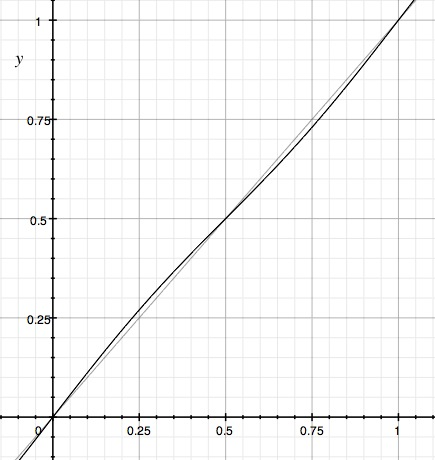
\includegraphics[scale=0.4]{sinewave}
\end{center}

\noindent Note that the two lines intersect at three points: \((0, 0), (\nicefrac{1}{2}, \nicefrac{1}{2})\) and \((1, 1)\). So if my credence in \(p\) is either 0, \(\nicefrac{1}{2}\) or 1, then my judgment is ratifiable. Otherwise, it is not. So the ratifiability constraint says that for any \(p\) about a baseball game, my credence in \(p\) should be either 0, \(\nicefrac{1}{2}\) or 1. But that's crazy. It's easy to imagine that I know (a) that in a particular game, the home team is much stronger than the away team, (b) that the stronger team usually, but far from always, wins baseball games, and (c) I'm systematically a little over-confident about my judgments about baseball games, in the way just described. In such a case, my credence that the home team will win should be high, but less than 1. That's just what the ratificationist denies is possible.

This kind of case proves that it isn't always rational to have ratifiable credences. It would take us too far afield to discuss this in detail, but it is interesting to think about the comparison between the kind of case I just discussed, and the objections to backwards induction reasoning in decision problems that have been made by Pettit and Sugden \citeyearpar{Pettit1989-PETTBI}, and by Stalnaker \citeyearpar{Stalnaker1996, Stalnaker1998}. The backwards induction reasoning they criticise is, I think, a development of the idea that decisions should be ratifiable. And the clearest examples of when that reasoning fails concern cases where there is a unique ratifiable decision, and it is guaranteed to be one of the worst possible outcomes. The example I described in the last few paragraphs has, quite intentionally, a similar structure.

The upshot of all this is that I think these regress arguments work. They aren't, I think, directly an argument against EW. What they are is an argument against the most promising way the EW theorist has for arguing that the table I started with misstates $S$'s epistemic situation. Given that the regress argument against JSE works though, I don't see any way of rescuing EW from this argument.
